\chapter{Evaluation}
\label{ch:study}

The scope of the user study was to collect data from participants simulating bruxism as well as performing contrast jaw movements. All of the sensors but the throat microphone were recorded with the RPI. The throat microphone was connected directly to the laptop used to control the RPI.

A total of 10 participants, 1 female, were recruited, with the youngest participant aged 19 and the oldest aged 28. After inspecting the data, 4 recordings of the temporalis muscles were removed from the resulting dataset (3 recordings of the left temporalis muscle, 1 recording of the right temporalis muscle). In one of the cases, the EMG electrodes disconnected themselves during the study. In the other cases, the data was very noisy. 2 audio recordings were also discarded. The challenges during the data collection are discussed in ch. \ref{ch:sensor_attachment}. 

The experiment took about 30min. The collected usable data had a length of about 16min. Throughout the experiment, the participants were asked to stand still if not asked otherwise, especially in the phase with the bruxism-related tasks, and to focus their eyes on a circle on the wall in front of them. At every step, they were instructed by the experimenter about the exercise they had to perform and the moment they had to start and stop performing it. An overview of the user study can be seen in figure \ref{image:study_overview}.

\begin{figure}[h]
\centering
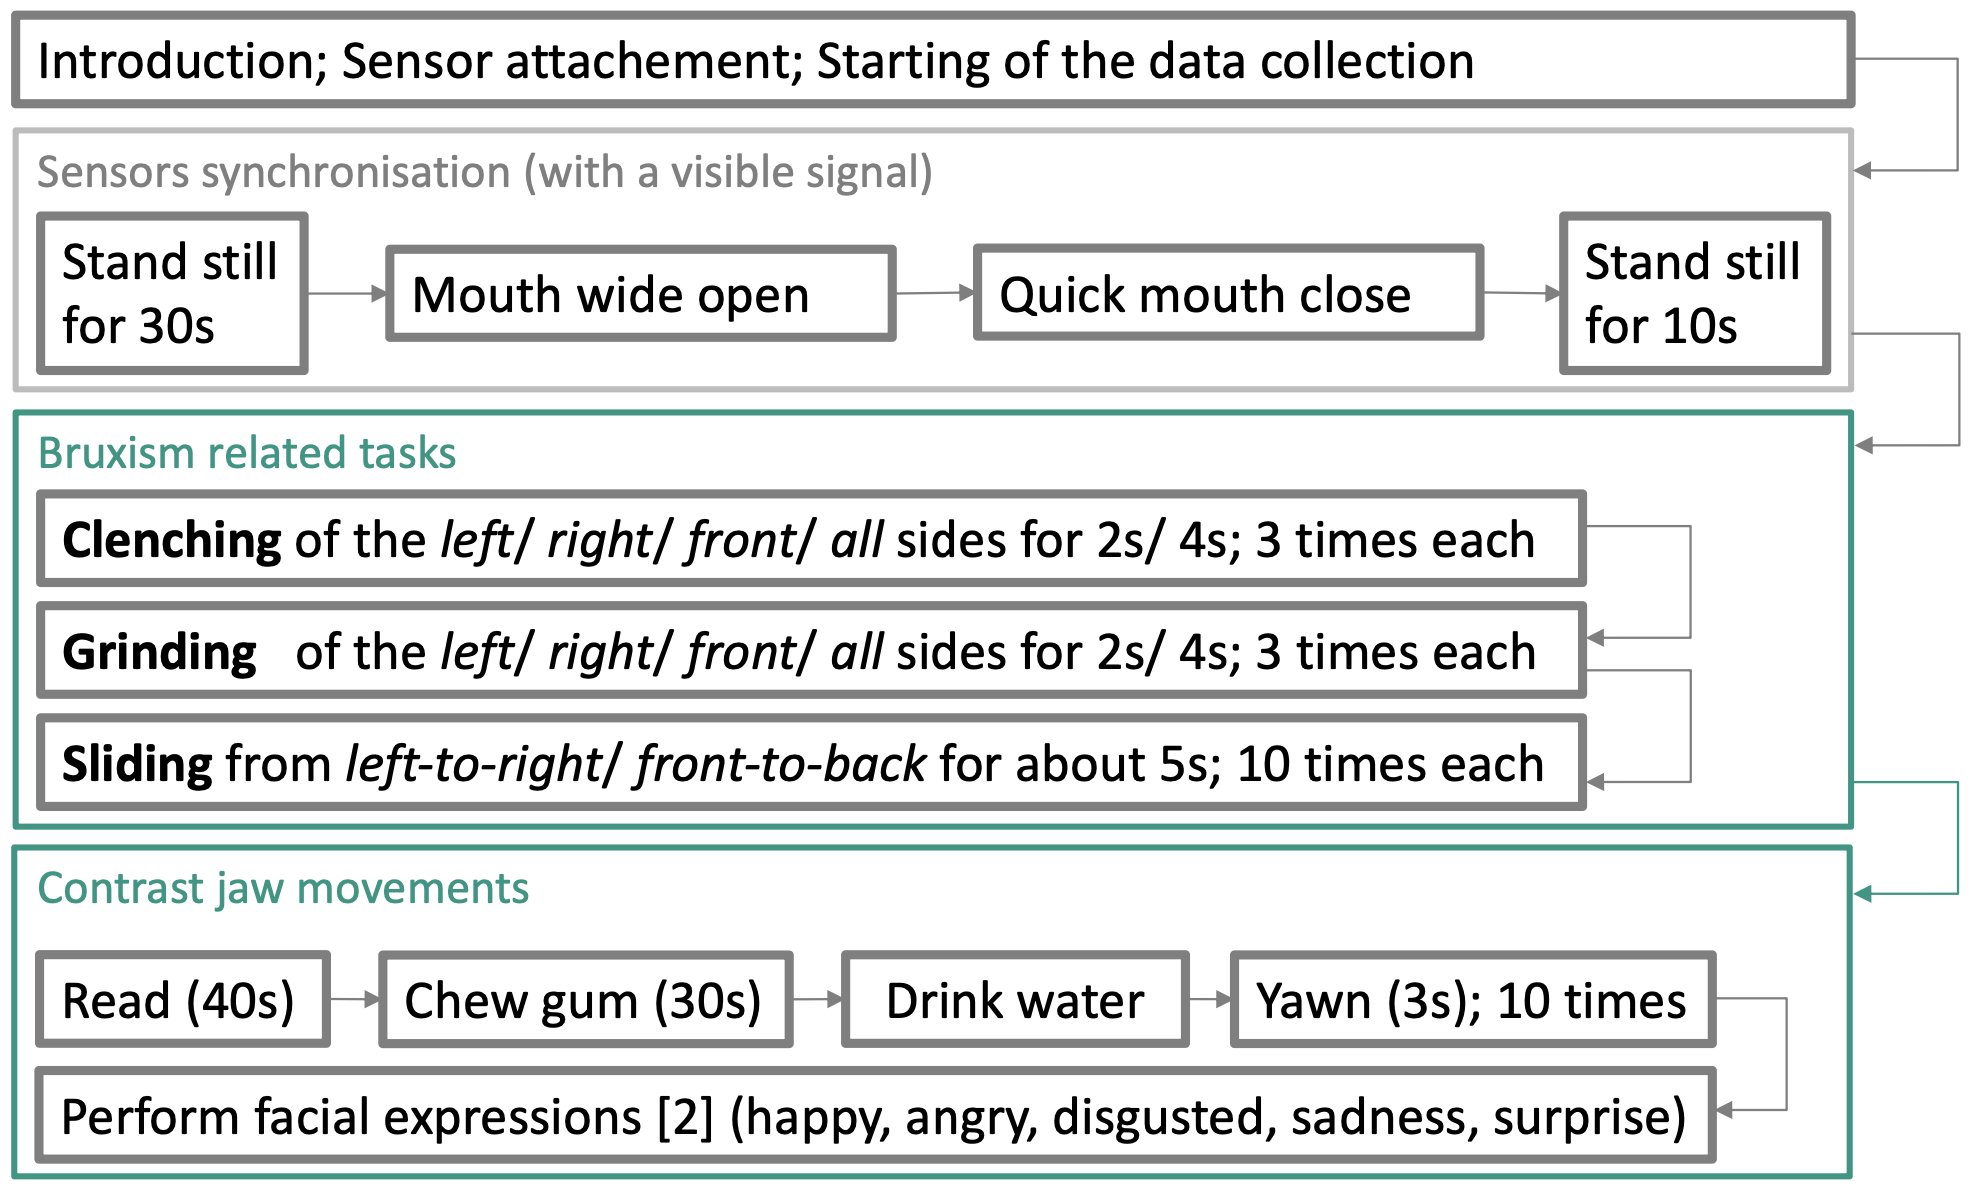
\includegraphics[width=0.8\textwidth]{src/media/study/study_overview.png}
\caption{User study overview}
\label{image:study_overview}
\end{figure}

\section{Data collection}

A total of 8 raw audio files were collected with the throat microphone. Six complete sets of time-series (a full set having N = 37 time-series) were used. In one set of time-series, the EMG recordings of the right temporalis muscle were corrupted (leaving n = 36 time-series). In the other three sets of time-series, the EMG recordings of the left temporalis muscle were corrupted (leaving n = 36 time-series for each set). The  study  yielded a total of 366 time-series collected with the RPI and eight audio recordings, with a total data removal of 1\% for the RPI (representing 10\% data removal of the collected EMG time-series) and 20\% for the audio recordings.

The time-series had a length of around 16min. The 37 time-series consists of the x, y, and z axis of the left (right) eSense earables gyroscope, x, y, and z axis of the left (right) eSense earables accelerometer, x, y, and z axis of the left (right) BNO055 gyroscope, x, y and z axis of the left (right) BNO055 accelerometer, w, x, y and z axis of the left (right) BNO055 quaternion, EMG signal for the left (right) masseter, left (right) temporalis, and GSR (table \ref{table:data_collection}).

\begin{table}[!h]
\centering
\begin{tabular}{|m{0.25\linewidth}|m{0.4\linewidth}|m{0.2\linewidth}|} 
 \hline
 Device & Time-series & Sample Rate \\ [0.5ex] 
 \hline\hline
 eSense earables &
        \begin{tabular}[t]{ll}
            Left gyroscope \texttt{x, y, z} \\
            Left accelerometer \texttt{x, y, z} \\
            \\
            Right gyroscope \texttt{x, y, z} \\
            Right accelerometer \texttt{x, y, z}
        \end{tabular} &
        \begin{tabular}[t]{ll}
            100Hz \\
            \\\\
            100Hz
        \end{tabular} \\
 \hline
 BNO055 &
        \begin{tabular}[t]{ll}
            Left gyroscope \texttt{x, y, z} \\
            Left accelerometer \texttt{x, y, z} \\
            Left quaternion \texttt{w, x, y, z} \\
            \\
            Right gyroscope \texttt{x, y, z} \\
            Right accelerometer \texttt{x, y, z} \\
            Right quaternion \texttt{w, x, y, z}
        \end{tabular} &
        \begin{tabular}[t]{ll}
            100Hz \\
            \\\\\\
            100Hz
        \end{tabular} \\
\hline
EMG &
        \begin{tabular}[t]{ll}
            Left masseter \\
            Right masseter \\
            Left temporalis \\
            Right temporalis
        \end{tabular} &
        \begin{tabular}[t]{ll}
            256Hz
        \end{tabular} \\
\hline
Throat Microphone &
        \begin{tabular}[t]{ll}
            Raw audio
        \end{tabular} &
        \begin{tabular}[t]{ll}
            44.1kHz
        \end{tabular} \\
\hline
GSR &
        \begin{tabular}[t]{ll}
            GSR
        \end{tabular} &
        \begin{tabular}[t]{ll}
            20Hz
        \end{tabular} \\
\hline
\hline
Total & 37 time-series \& 1 audio file & \\
\hline
\end{tabular}
\caption{Collected data overview}
\label{table:data_collection}
\end{table}


\section{Sensor Attachment}
\label{ch:sensor_attachment}

The sensor attachment was done as described in the table \ref{table:hardware_peripherals}. Some of the peripherals required special mounting based on the participants anatomy (see \ref{par:emg_attachment}) and some of the participants had trouble wearing some types of peripherals (see \ref{par:esense_attachment}, \ref{par:mic_attachment}).

\section{Study Design}

The participants were introduced to the user study and the concept of bruxism. After generating a pseudo-random code-name and acknowledging and accepting the terms of the data collection the sensors were attached and the data collection started.

\subsection{Sensor synchronization}
Even though the RPI already synchronizes the collected data from the connected sensors, using its internal clock, the throat microphone was connected to a separate device. To be able to align these time-series later, the participants were asked to perform a certain jaw movement, as a synchronization signal:
\begin{enumerate}
    \item Stand still for 30s;
    \item Mouth wide open;
    \item Quick mouth close;
    \item Stand still for 10s.
\end{enumerate}

\subsection{Bruxism related tasks}
In this phase the participants were asked to perform the following jaw movements to simulate bruxism:
\begin{itemize}
    \item \textbf{Clenching}: touch the requested sides with as much force as possible, without other jaw movements.
    \item \textbf{Grinding}: touch the requested sides with as much force as possible, with additional small jaw movements. Imagine that you are rubbing the touching teeth with one another;
    \item \textbf{Sliding}: move your lower jaw in the requested pattern.
\end{itemize}

The sequence of performing of these movements was repeated several times with different duration:
\begin{enumerate}
    \item Clench the \emph{left} side for \textbf{2s}, 3 times in total, with pauses in-between;
    \item Clench the \emph{right} side for \textbf{2s}, 3 times in total, with pauses in-between;
    \item Clench the \emph{front} side for \textbf{2s}, 3 times in total, with pauses in-between;
    \item Clench \emph{all sides} for \textbf{2s}, 3 times in total, with pauses in-between;
    \item pause for 5s.
    \item Clench the \emph{left} side for \textbf{4s}, 3 times in total, with pauses in-between;
    \item Clench the \emph{right} side for \textbf{4s}, 3 times in total, with pauses in-between;
    \item Clench the \emph{front} side for \textbf{4s}, 3 times in total, with pauses in-between;
    \item Clench \emph{all sides} for \textbf{4s}, 3 times in total, with pauses in-between;
\end{enumerate}

Similarly grinding was done next.

Then sliding was performed with the movement of the whole jaw:
\begin{enumerate}
    \item Slide from \emph{left-to-right} for about \textbf{5s}, 10 times in total;
    \item Slide from \emph{front-to-back} for about \textbf{5s}, 10 times in total;
\end{enumerate}

\subsection{Contrast jaw movements}
After the bruxism phase, it was important to record other typical jaw movements. For that following materials were prepared:
\begin{itemize}
    \item A text snippet (in both English and German language), with a time-to-read of about 40s;
    \item Chewing gum;
    \item A glass of water;
    \item 6 facial expressions from the KDEF \cite{lundqvist1998karolinska}, printed on paper.
\end{itemize}

The tasks were then done in the following order:
\begin{enumerate}
    \item Read the following text out loud, either in English or German;
    \item Chew a gum for \textbf{30s};
    \item Drink a glass of water;
    \item Yawn for about \textbf{3s} or longer if you feel so, 10 times in total;
    \item Perform the following facial expression as you see it for about \textbf{4s}, relax your face, and proceed with the next facial expression, 12 times in total.
\end{enumerate}

After that, the data collection was stopped. The raw audio data was saved on the laptop and the generated \texttt{.csv} files were copied from the RPI to the laptop using \texttt{scp}. The whole user study duration was about 35min.


\section{Survey}

Each participant completed a survey at the end of the user study. This included demographic questions and questions about the wear and feel of the peripherals. The results are presented in the table \ref{table:masseter_asymmetry}, \ref{table:devices_comfort} and \ref{table:devices_score}. It appears that the participants found the BNO055s the most comfortable.

\begin{table}[!h]
\centering
\begin{tabular}{|>{\raggedright}m{0.4\linewidth}||m{0.11\linewidth}|m{0.11\linewidth}|m{0.11\linewidth}|m{0.11\linewidth}|} 
 \hline
  & Std. dev. & Var. & Min & Max \\ [0.5ex] 
 \hline\hline
 Visible difference between masseter muscles & 1.12 & 1.06 & -2 & 2 \\
 \hline
\end{tabular}
\caption{Masseter muscle asymmetry (-2 = left side is bigger, 2 = right side is bigger)}
\label{table:masseter_asymmetry}
\end{table}

\begin{table}[!h]
\centering
\begin{tabular}{|>{\raggedright}m{0.4\linewidth}||m{0.11\linewidth}|m{0.11\linewidth}|m{0.11\linewidth}|m{0.11\linewidth}|} 
 \hline
  & Std. dev. & Var. & Min & Max \\ [0.5ex] 
 \hline\hline
 Throat microphone & 1.07 & 1.03 & 0 & 3 \\
 \hline
 eSense earables & 0.77 & 0.88 & 0 & 3 \\
 \hline
 EMG electrodes & 0.28 & 0.53 & 2 & 3 \\
 \hline
 BNO055 & 0.28 & 0.53 & 2 & 3 \\
 \hline
\end{tabular}
\caption{Participants opinion on the devices comfort (0 = very uncomfortable, 3 = very comfortable).}
\label{table:devices_comfort}
\end{table}

\begin{table}[!h]
\centering
\begin{tabular}{|>{\raggedright}m{0.4\linewidth}||m{0.11\linewidth}|m{0.11\linewidth}|m{0.11\linewidth}|m{0.11\linewidth}|} 
 \hline
  Device & Std. dev. & Var. & Min & Max \\ [0.5ex] 
 \hline\hline
 Throat microphone & 0.12 & 0.02 & 0.70 & 0.97 \\
 \hline
 eSense earables & 0.10 & 0.01 & 0.71 & 1 \\
 \hline
 EMG electrodes & 0.17 & 0.03 & 0.43 & 1 \\
 \hline
 BNO055 & 0.10 & 0.01 & 0.75 & 1 \\
 \hline
\end{tabular}
\caption{Device score based on participants' answers on overall wear and feel (0 = lowest score, 1 = highest score).}
\label{table:devices_score}
\end{table}

\section{Analysis}
\label{ch:methodology}

\subsection{Labeling}

\paragraph{Data irregularity}

The sensors are set to deliver data at a predefined sample rate. But in practice, this value fluctuates somewhat. As a result, the datapoints of the collected time-series are not aligned. Even the data of a single time-series may be captured at different intervals while maintaining the designed sample rate. In such cases, the data we deal with is \emph{irregular} (e.g. \ref{image:irregular-data}).

To remove the irregularity from the data and make it \emph{regular}, the time-series can be resampled (e.g. \ref{image:regular-data}). At this moment, we can choose the resampling rate equal to the original sampling rate (i.e., aligning the datapoints of a time-series to fixed intervals) or select a higher or lower sample rate. As we don't require high-precision timestamps in the nanoseconds range, it is enough to have precision in the tens or hundreds of milliseconds. After some trials, the datasets were resampled to 20Hz. The missing values were linearly interpolated.

\begin{figure}[!h]
\centering
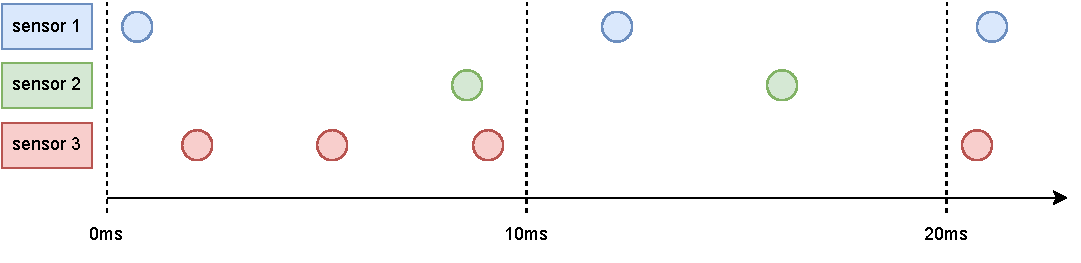
\includegraphics[width=\textwidth]{src/media/methodology/irregular-data2.pdf}
\caption{Example of irregular data. Circles represent the moment a payload was captured. Colors relate the point in time to the sensor of origin}.
\label{image:irregular-data}
\end{figure}

\begin{figure}[!h]
\centering
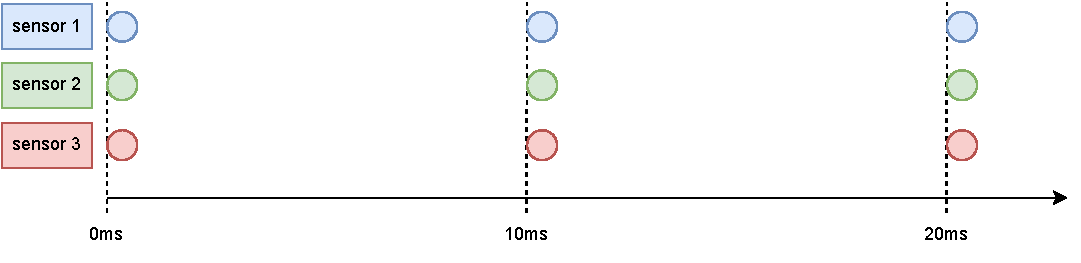
\includegraphics[width=\textwidth]{src/media/methodology/regular-data.pdf}
\caption{Example of regular data. Circles represent the moment a payload was captured. Colors relate the point in time to the sensor of origin}.
\label{image:regular-data}
\end{figure}

\paragraph{Label methodology}

The labeling was done manually after the user study concluded. To ease this process, the following procedure was done:

\begin{enumerate}
    \item For each dataset, the maximum of the minimum timestamps was calculated (i.e., the first timestamp of the last sensor that started delivering data). Then all timestamps in a dataset were offset by the calculated timestamp. As a result, if plotted, having the time on the X-axis, the time-series will start at 0.
    \item The values for each time-series were z-normalized, and the plots were presented overlapping in a single figure (one of such datasets is shown in fig. \ref{image:dataset_overview}).
\end{enumerate}

To z-normalize the values for each time-series the following formula was used:

\[ y := \frac{y - \mu}{\sigma} \]

where $y$ is a value in the time-series, $\mu$ is the mean, and $\sigma$ is the standard deviation. 

The data aligned perfectly, and different activity types performed during the user study can be precisely located.

\paragraph{Label types}

All the time ranges with the bruxism-related tasks were labeled as 1 (i.e., is bruxism). The rest of the datapoints else was labeled as 0 (i.e., no bruxism).

\paragraph{Window selection}

A sliding window approach was applied, which is the standard procedure in time-series data processing. The sliding window had a length of 1.6s with 50\% overlap (0.8s). This ensures that we are grouping enough data points together and not missing transitions between muscle contractions or contraction bursts. The window was labeled by the dominant event in that window; If the larger portion of the window contains bruxism data and a smaller portion of silent data, the window would be labeled as bruxism. If the split is equal, then the window is labeled as silent \cite{bondareva2021earables}.

This resulted in windows having 32 datapoints for each of the 37 time-series, yielding 1184 features.

\subsection{Classification}

The classification was done by using a brute-force approach. Four traditional machine learning classifiers from sklearn were trained: random forest (RF), k-nearest neighbors (kNN), support vector machine (SVM), and decision tree (DT).

\paragraph{Brute-force Approach Overview}

The time-series were generalized into the following groups:

\begin{listing}[!h]
\begin{minted}
[
frame=lines,
framesep=2mm,
baselinestretch=1.2,
fontsize=\footnotesize,
linenos,
breaklines
]
{python}
timeseries_groups = {
    "bno_gyro": ['x28_gyro_x', 'x28_gyro_y', 'x28_gyro_z', "x29_gyro_x", "x29_gyro_y", "x29_gyro_z"],
    "bno_acc": ["x28_acceleration_x", "x28_acceleration_y", "x28_acceleration_z", "x29_acceleration_x", "x29_acceleration_y", "x29_acceleration_z"],
    "bno_quat": ["x28_quaternion_w", "x28_quaternion_x", "x28_quaternion_y", "x28_quaternion_z", "x29_quaternion_w", "x29_quaternion_x", "x29_quaternion_y", "x29_quaternion_z"],

    "ble_gyro": ["gyro_x", "gyro_y", "gyro_z", "gyro_x_2", "gyro_y_2", "gyro_z_2"],
    "ble_acc": ["acceleration_x", "acceleration_y", "acceleration_z", "acceleration_x_2", "acceleration_y_2", "acceleration_z_2"],

    "gsr": ["gsr"],

    "masseter": ["masseter_left", "masseter_right"],

    "temporalis": ["temporalis_left", "temporalis_right"]
}
\end{minted}
\caption{Dataset time-series abstractions}
\label{listing:dataset_abstractions}
\end{listing}

then a power set (excluding the empty set) was computed for the set of the groups of time-series: \texttt{"bno\_gyro", "bno\_acc", "bno\_quat", "ble\_gyro", "ble\_acc", "gsr", "masseter", "temporalis"} (8 in total). For every two-sided sensor, both sides were placed in the same group. Bruxers tend to have one side of the masticatory muscles overdeveloped, which will lead to cleaner data samplings and better results. But this is highly individual, and to cover every possible use-case scenario, the data from both sides is needed.

The resulted power set had a length of 255 (\(2^8 - 1\))

For Every such group, an array of windows with the corresponding time-series from every dataset was computed. The window labels from every dataset were stored in an array as well so that a window will share the same positional index in the array as its label does.

\paragraph{Brute-force training}

Every feature set (group of time-series) windows were split in 20:80 ratio (20 for testing, 80 for training) and passed sequentially to a model classifier.

\paragraph{Brute-force evaluation}

For every model---feature-set pair, an accuracy score was calculated.
